\documentclass[12pt]{beamer}
\usepackage[utf8]{inputenc}
\usepackage[spanish]{babel}
\usepackage{color}
\usepackage{hyperref}
\usepackage{amsmath}
\usepackage{amsthm}
\usepackage{multicol}
\usepackage{graphicx}
\usepackage{tikz}
\usepackage[autostyle,spanish=mexican]{csquotes}
%\usepackage[sfdefault]{roboto}  %% Option 'sfdefault' only if the base font of the document is to be sans serif
\renewcommand{\arraystretch}{1.5}
\renewcommand{\rmdefault}{cmr}% cmr = Computer Modern Roman
\usefonttheme[onlymath]{serif}

\newcommand{\python}{\texttt{python}}
\newcommand{\textoazul}[1]{\textcolor{blue}{#1}}
\newcommand{\azulfuerte}[1]{\textcolor{blue}{\textbf{#1}}}
\newcounter{saveenumi}
\newcommand{\seti}{\setcounter{saveenumi}{\value{enumi}}}
\newcommand{\conti}{\setcounter{enumi}{\value{saveenumi}}}

\linespread{1.5}
\beamertemplatenavigationsymbolsempty
\usefonttheme{professionalfonts}
\usefonttheme{serif}
\DeclareGraphicsExtensions{.pdf,.png,.jpg}
\renewcommand {\arraystretch}{1.25}
\mode<presentation>
{
  \usetheme{Warsaw}
  \setbeamertemplate{headline}{}
  %\useoutertheme{infolines}
  \useoutertheme{default}
  \setbeamercovered{invisible}
  % or whatever (possibly just delete it)
  \setbeamertemplate{section in toc}[sections numbered]
  \setbeamertemplate{subsection in toc}[subsections numbered]
  \setbeamertemplate{subsection in toc}{\leavevmode\leftskip=3.2em\rlap{\hskip-2em\inserttocsectionnumber.\inserttocsubsectionnumber}\inserttocsubsection\par}
  \setbeamercolor{section in toc}{fg=blue}
  \setbeamercolor{subsection in toc}{fg=blue}
  \setbeamercolor{frametitle}{fg=yellow}

  \setbeamertemplate{footline} 
{
  \leavevmode%
  \hbox{%
  \begin{beamercolorbox}[wd=.333333\paperwidth,ht=2.25ex,dp=1ex,center]{author in head/foot}%
    \usebeamerfont{author in head/foot}\insertsection
  \end{beamercolorbox}%
  \begin{beamercolorbox}[wd=.333333\paperwidth,ht=2.25ex,dp=1ex,center]{title in head/foot}%
    \usebeamerfont{title in head/foot}\textcolor{yellow}{\insertsubsection}
  \end{beamercolorbox}%
  \begin{beamercolorbox}[wd=.333333\paperwidth,ht=2.25ex,dp=1ex,right]{date in head/foot}%
    \usebeamerfont{date in head/foot}\insertshortdate{}\hspace*{2em}
    \insertframenumber{} / \inserttotalframenumber\hspace*{2ex} 
  \end{beamercolorbox}}%
  \vskip0pt%
}
}
\makeatother

\makeatletter
\patchcmd{\beamer@sectionintoc}
  {\vfill}
  {\vskip\itemsep}
  {}
  {}
\makeatother
\title{\large{Tema 1 - Escalas, condición y estabilidad}}
\subtitle{Curso de Física Computacional}
\author[]{M. en C. Gustavo Contreras Mayén}
\date{\today}
\institute{Facultad de Ciencias - UNAM}
\titlegraphic{\includegraphics[width=2cm]{Imagenes/escudo-facultad-ciencias}\hspace*{4.75cm}~%
   \includegraphics[width=2cm]{Imagenes/escudo-unam}
}
\begin{document}
\maketitle
\section*{Contenido}
\frame[allowframebreaks]{\tableofcontents[currentsection, hideallsubsections]}
\fontsize{14}{14}\selectfont
\spanishdecimal{.}
\section{Punto flotante}
\frame{\tableofcontents[currentsection, hideothersubsections]}
\begin{frame}
\frametitle{Introducción}
La aritmética que se realiza en una computadora es distinta a la aritmética que hemos aprendido de los cursos de álgebra o cálculo.
\\
\bigskip
\pause
Uno pensaría que siempre serían verdaderas las siguientes operaciones:
\begin{itemize}
\item $2 + 2 = 4$
\item $4 * 4 = 16$
\item $(\sqrt{3})^{2} = 3$
\end{itemize}
Sin embargo, la tercera  operación no siempre se da.
\end{frame}
\begin{frame}
\frametitle{Introducción}
En nuestro mundo matemático se permiten y se manejan  números expresados con una cantidad infinita de cifras.
\\
\bigskip
\pause
Sin embargo, en el mundo computacional, cada número representable tiene sólo un número finito de cifras. Esto significa que sólo los números enteros y algunos números racionales se pueden presentar con exactitud. 
\end{frame}
\begin{frame}
\frametitle{Introducción}
Puesto que el número $\sqrt{3}$ no es racional, la computadora le da una representación aproximada, cuyo cuadrado no es $3$, aunque si lo bastante cercano a $3$ para que sea aceptable en la mayor parte de las situaciones.
\end{frame}
\subsection{Números de punto flotante}
\begin{frame}
\frametitle{Representación de punto flotante}
Todos los números deben ser almacenados en la computadora de tal manera que las operaciones aritméticas puedan ejecutarse  con estos números.
\\
\bigskip
\pause
La mayoría de las computadoras tiene dos maneras de guardar estos números:
\setbeamercolor{item projected}{bg=blue!70!black,fg=yellow}
\setbeamertemplate{enumerate items}[circle]
\begin{enumerate}[<+->]
\item Formato de enteros.
\item Formato de punto flotante.
\end{enumerate}
\end{frame}
\begin{frame}
\frametitle{Representación de punto flotante}
Los número enteros son relativamente directos, en donde debemos de considerar el intervalo que se puede representar.
\\
\bigskip
\pause
El formato punto flotante es una forma más general permitiendo almacenar números que no son enteros, revisaremos el formato estándar de representación.
\end{frame}
\begin{frame}
\frametitle{Punto flotante para decimales}
Consideremos un número $x$ distinto de cero, escrito en el sistema decimal de manera única como:
\begin{align*}
x =  \sigma \cdot \overline{x} \cdot 10^{e}
\end{align*}
\pause
donde: 
\begin{itemize}
\item El \textcolor{red}{signo} es $\sigma= \pm 1$,
\item El \textcolor{blue}{exponente} $e$ es un entero.
\item La \textcolor{ao}{mantisa} es tal que $ 1 \leq \overline{x} \leq 10$.
\end{itemize}
\end{frame}
\begin{frame}
\frametitle{Ejemplo de representación}
Consideremos el número
\begin{align*}
123.45 = +1 \cdot (1.2345) \cdot 10^{2}
\end{align*}
\pause
Entonces:
\begin{itemize}
\item El signo es $\sigma = +1$
\item El exponente es $e = 2$
\item La mantisa es $\overline{x} =1.2345$
\end{itemize}
\end{frame}
\begin{frame}
\frametitle{Punto flotante en binario}
El sistema binario representa los número como una suma de múltiplos enteros de potencias de $2$.
\\
\bigskip
\pause
La base del sistema binario son los dígitos $0$ y $1$.
\end{frame}
\begin{frame}
\frametitle{Ejemplo de Representación}
El siguiente número $x$ en binario tiene el valor en el sistema decimal como:
\begin{align*}
(1101.11)_{2} &= 1 \cdot 2^{3} + 1 \cdot 2^{2} + 0 \cdot 2^{1} + 1 \cdot 2^{0} + \\
 &+ 1 \cdot 2^{-1} + 1 \cdot 2^{-2}
\end{align*}
\end{frame}
\begin{frame}
\frametitle{Representación de punto flotante en binario}
Consideremos el número $x$ escrito en forma binaria, de manera análoga como en el caso decimal:
\begin{align*}
x =  \sigma \cdot \overline{x} \cdot 2^{e}
\end{align*}
\pause
donde: 
\begin{itemize}
\item El \textcolor{red}{signo} es $\sigma= \pm 1$,
\item El \textcolor{blue}{exponente} $e$ es un entero.
\item La \textcolor{ao}{mantisa} es una fracción binaria tal que $ (1)_{2} \leq \overline{x} \leq (10)_{2}$.
\end{itemize}
\end{frame}
\begin{frame}
\frametitle{Ejemplo de un número de punto flotante}
Sea el número
\begin{align*}
x = (11011.0111)_{2} = +1 \cdot (1.10110111)_{2} \cdot 2^{4}
\end{align*}
\pause
Entonces
\begin{itemize}
\item El signo es $\sigma = +1$
\item El exponente es $e = 4 = (100)_{2}$
\item La mantisa es $\overline{x} = (1.10110111)_{2}$
\end{itemize}
\end{frame}
\begin{frame}
\frametitle{Dos observaciones}
\setbeamercolor{item projected}{bg=blue!70!black,fg=yellow}
\setbeamertemplate{enumerate items}[circle]
\begin{enumerate}[<+->]
\item Para todo número $x \neq 0$, el primer dígito de la izquierda del punto en $\overline{x}$, es siempre $1$.
\item La representación de $x$ también está sujeta al número de dígitos binarios en $\overline{x}$ y en el tamaño del exponente.
\end{enumerate}
\end{frame}
\section{Precisión en punto flotante}
\frame{\tableofcontents[currentsection, hideothersubsections]}
\subsection{Definición de precisión}
\begin{frame}
\frametitle{Definición}
El número permitido de dígitos binarios en $\overline{x}$ se le llama \textcolor{blue}{precisión} de la representación de punto flotante binario.
\end{frame}
\subsection{Estándar IEEE 754}
\begin{frame}
\frametitle{El Estándar IEEE 754}
El estándar IEEE 754 para la aritmética de punto flotante es el formato para números puntos flotante usado en computación.
\\
\bigskip
Este estándar maneja dos tipos de precisión: simple y doble.
\end{frame}
\subsection{Precisión simple}
\begin{frame}
\frametitle{Precisión simple}
En este estándar, la representación de \emph{punto flotante de precisión simple} de un número $x$, tiene una precisión de $24$ dígitos binarios y el exponente está limitado a $-126 \leq e \leq 127$
\begin{align*}
x = \sigma \cdot (1.a_{1} \, a_{2} \, \ldots \, a_{22} \, a_{23}) \cdot 2^{e}
\end{align*}
En binario
\begin{align*}
-(1111110)_{2} \leq e \leq (1111111)_{2}
\end{align*}
\end{frame}
\begin{frame}
\frametitle{Posición de los bits}
Este formato usa $4$ bytes ($32$  bits), distribuidos de la siguiente manera:
\begin{figure}
    \centering
    \includegraphics[scale=1.2]{Imagenes/precision_simple.eps}
\end{figure}
\end{frame}
\begin{frame}
\frametitle{Posición de los bits}
\begin{figure}
    \centering
    \includegraphics[scale=1.2]{Imagenes/precision_simple.eps}
\end{figure}
\begin{itemize}[<+->]
\item El signo $\sigma$ se almacena en el bit $b_{1}$, tal que $b_{1} = 0$ para $\sigma = +1$ y $b_{1} = 1$ para $\sigma = -1$
\end{itemize}
\end{frame}
\begin{frame}
\frametitle{Posición de los bits}
\begin{figure}
    \centering
    \includegraphics[scale=1.2]{Imagenes/precision_simple.eps}
\end{figure}
\begin{itemize}[<+->]
\item Se define $E = e + 127$ como el valor del exponente desplazado $127$ lugares.
\item Se almacena el entero binario positivo $E$ en los bits $b_{2}$ a $b_{9}$
\end{itemize}
\end{frame}
\begin{frame}
\frametitle{Posición de los bits}
\begin{figure}
    \centering
    \includegraphics[scale=1.2]{Imagenes/precision_simple.eps}
\end{figure}
\begin{itemize}[<+->]
\item El número binario $a_{1} \, a_{2} \ldots a_{23}$ se almacena en los bits $b_{10}$ a $b_{32}$
\end{itemize}
\end{frame}
\begin{frame}
\frametitle{Observaciones al formato}
El primer dígito binario $1$ de $\overline{x}$ no es guardado en la representación de punto flotante cuando el número se almacena en memoria, pero éste dígito se agrega en $\overline{x}$ cuando el número de punto flotante es llamado de la memoria para ejecutar alguna operación aritmética.
\end{frame}
\begin{frame}
\frametitle{Observaciones al formato}
Se requiere de una representación especial del número $x = 0$, se almacena como:
\begin{itemize}
\item $\sigma = 0$
\item $exponente = 0$
\item $b_{1} \, b_{2} \, \ldots \, b_{32} = (00 \ldots 0)_{2}$
\end{itemize}
\end{frame}
\begin{frame}
\frametitle{Observaciones al formato}
En precisión simple, el número 1 se representa por
\begin{align*}
1.00000000000000000000000
\end{align*}
\pause
El siguiente número binario más grande es
\begin{align*}
1.00000000000000000000001
\end{align*}
siendo $1$ el dígito binario en la posición $23$ en la parte derecha del punto.
\end{frame}
\begin{frame}
\frametitle{Observaciones al formato}
El épsilon de la máquina es $2^{-23}$, entonces tenemos que
\begin{align*}
2^{-23} \simeq \num{1.19d-7}
\end{align*}
\pause
Por lo que con el formato de precisión simple del estándar IEEE 754, se pueden aproximar $7$ dígitos decimales de un número $x$ cuando se escribe en su formato decimal.
\end{frame}
\subsection{Precisión doble}
\begin{frame}
\frametitle{Definición de la precisión doble}
La representación de \emph{punto flotante de precisión doble} del estándar IEEE 754 de un número $x$, tiene una precisión de $53$ dígitos binarios, y el exponente está limitado a $-1022 \leq e \leq 1023$.
\begin{align*}
x = \sigma \cdot (1.a_{1} \, a_{2} \, \ldots \, a_{51} \, a_{52}) \cdot 2^{e}
\end{align*}
\end{frame}
\begin{frame}
\frametitle{Posición de los bits}
La precisión doble utiliza $8$ bytes ($64$ bits) y los números se almacenan de la siguiente forma:
\begin{figure}
    \centering
    \includegraphics[scale=1.2]{Imagenes/precision_doble.eps}
\end{figure}
\vspace*{-1cm}
Los bits son guardados de manera análoga a la precisión simple, pero con $E = e + 1023$
\end{frame}
\begin{frame}
\frametitle{Observaciones a la precisión doble}
El épsilon de la máquina en precisión doble es
\begin{align*}
2^{-52} \simeq \num{2.22d-16}
\end{align*}
\pause
Con el formato de precisión doble del estándar IEEE 754 se puede utilizar para guardar aproximadamente 16 dígitos de un número $x$.
\end{frame}
\begin{frame}
\frametitle{Casos especiales del estándar IEEE 754}
Veamos algunos casos especiales de combinaciones entre el signo $(-1)^{s}$, el exponente $e$ y la mantisa $f$:
\pause
\begin{table}
\fontsize{10}{10}\selectfont
\begin{tabular}{l c c}
\hline
Nombre del número & Valores de $\sigma$, $e$, $f$ & Valor \\ \hline
Normal & $0 < e < 255$ & $(-1)^{s} \times 2^{e-127} \times 1.f$ \\ \hline
Subnormal & $e = 0, f \neq 0$ & $(-1)^{s} \times 2^{e-126} \times 0.f$ \\ \hline
Signo cero $(\pm 0)$ & $e = 0, f = 0$ & $(-1)^{s} \times 0.0$ \\ \hline
$+ \infty$ & $s = 0, e=255, f = 0$ & \textbf{\texttt{+INF}} \\ \hline
$- \infty$ & $s = 1, e=255, f = 0$ & \textbf{\texttt{-INF}} \\ \hline
Not a number & $s = u, e=255, f \neq 0$ & \textbf{\texttt{NaN}} \\ \hline
\end{tabular}
\end{table}
\end{frame}
\begin{frame}
\frametitle{Números normales}
Los números normales tienen un valor entre $0 < e < 255$, y con ellos la convención es suponer que el primer bit de la mantisa es un $1$.
\\
\bigskip
De modo que sólo se almacena la parte fraccional $f$ después del punto binario. 
\end{frame}
\begin{frame}
\frametitle{Valores $\pm \: \text{INF}$ y $NaN$ }
Nótese que los valores $\pm \: \text{INF}$ y $\text{NaN}$ no son números en el sentido matemático, es decir, son objetos que pueden ser manipulados o utilizados en cálculos para tomar límites.
\\
\bigskip
\pause
Más bien, son señales para la computadora y para el usuario de que algo ha ido mal y que el cálculo probablemente debería detenerse hasta resolver las cosas.
\end{frame}
\begin{frame}
\frametitle{Los valores $\pm 0$}
En contraste, el valor $-0$ se puede utilizar en un cálculo sin problemas.
\\
\bigskip
Algunos lenguajes pueden establecer variables no asignadas como $-0$ como una pista de que aún no se han asignado, pero no es lo más conveniente.
\end{frame}
\begin{frame}
\frametitle{Precisión relativa en punto flotante}
Debido a que la incertidumbre (error) está presente sólo en la mantisa y no en el exponente, las representaciones IEEE aseguran que todos los números normales de punto flotante tengan la misma precisión relativa.
\end{frame}
\begin{frame}
\frametitle{El bit fantasma}
Debido a que el primer bit se supone que es $1$, no tiene que ser almacenado, y los diseñadores de computadoras sólo necesitan recordar que hay un \emph{bit fantasma} allí para obtener un poco más de precisión.
\end{frame}
\begin{frame}
\frametitle{El primer bit}
Durante el procesamiento de números en un cálculo, el primer bit de un resultado intermedio puede llegar a ser cero, pero éste se cambia antes de que se almacene el número final.
\\
\bigskip
Para repetir, en los casos normales, la mantisa real ($1.f$ en notación binaria) contiene un $1$ implícito que precede al punto binario.
\end{frame}
\begin{frame}
\frametitle{El número de sesgo}
Con el fin de garantizar que el exponente $e$ almacenado sea siempre positivo, se agrega un número fijo llamado \textoazul{sesgo} al exponente real $p$, antes de que se almacene como exponente $e$.
\\
\bigskip
El exponente real, que puede ser negativo, es
\begin{equation}
p = e - \text{sesgo}
\label{eq:ecuacion_01_03}
\end{equation}
\end{frame}
\section{Modelos para el desastre}
\frame{\tableofcontents[currentsection, hideothersubsections]}
\subsection{Cancelación en la sustracción}
\begin{frame}
\frametitle{Cancelación en la sustracción}
Un cálculo que utiliza números que se almacenan de manera aproximada en la computadora, puede devolver una solución aproximada.
\\
\bigskip
Para demostrar este hecho, consideremos que hay un valor de incertidumbre, sea $x_{c}$ el valor representado en la computadora del valor exacto $x$, tal que:
\begin{equation}
x_{c} \simeq  x( 1 + \varepsilon_{x})
\label{eq:ecuacion_02_05}
\end{equation}
\end{frame}
\begin{frame}
\frametitle{Cancelación en la sustracción}
\begin{equation*}
x_{c} \simeq  x( 1 + \varepsilon_{x})
\end{equation*}
Donde $\epsilon_{x}$ es el error relativo de $x_{c}$, el cual se espera que sea similar en magnitud al épsilon de la máquina $\epsilon_{m}$.
\end{frame}
\begin{frame}
\frametitle{Cancelación en la sustracción}
Si usamos ésta notación para una diferencia entre dos valores $a = b - c$, tenemos que:
\begin{align}
\begin{aligned}
a = b - c & \Rightarrow a_{c} \simeq b_{c} - c_{c} \simeq \\
 &\simeq b \, (1 + \epsilon_{b}) - c \, (1 + \epsilon_{c}) \\
{} & \Rightarrow \dfrac{a_{c}}{a} \simeq 1 + \epsilon_{b} \dfrac{b}{a} - \dfrac{c}{a} \epsilon_{c}
\end{aligned}
\label{eq:ecuacion:02_06}
\end{align} 
\end{frame}
\begin{frame}
\frametitle{Cancelación en la sustracción}
Vemos que el error resultante en $a$ es un promedio de los errores en $b$ y $c$, y no hay seguridad en que los dos términos se cancelen.
\end{frame}
\begin{frame}
\frametitle{Cancelación en la sustracción}
El error en $a_{c}$ se incrementa cuando se restan dos valores cercanos $(b \simeq c)$, porque entonces estamos restando las partes más significativas de ambos números y dejando las partes menos significativas propensas a errores:
\pause
\begin{align}
\begin{aligned}
\dfrac{a_{c}}{a} &\stackrel{def}{=} 1 + \epsilon_{a} \simeq  \\
&\simeq 1 + \dfrac{b}{a}(\epsilon_{b} - \epsilon_{c}) \simeq  \\
&\simeq 1 + \dfrac{b}{a} \: \max(\abs{\epsilon_{b}}, \abs{\epsilon_{c}})
\end{aligned}
\label{eq:ecuacion_02_07}
\end{align}
\end{frame}
\begin{frame}
\frametitle{Cancelación en la sustracción}
\begin{align*}
\dfrac{a_{c}}{a} \simeq 1 + \dfrac{b}{a} \: \max(\abs{\epsilon_{b}}, \abs{\epsilon_{c}})
\end{align*}
Esto muestra que incluso si los errores relativos en $b$ y $c$ pueden cancelar algo, se multiplican por número grande $b / a$, lo que puede aumentar significativamente el error.
\end{frame}
\begin{frame}
\frametitle{Cancelación en la sustracción}
Debido a que no podemos asumir ningún signo de los errores, debemos asumir el peor escenario: el máximo en la expresion:
\begin{align*}
\dfrac{a_{c}}{a} \simeq 1 + \dfrac{b}{a} \: \max(\abs{\epsilon_{b}}, \abs{\epsilon_{c}})
\end{align*}
\end{frame}
\subsection{Ejercicio 1}
\begin{frame}
\frametitle{Ejercicio 1 - Ecuación cuadrática}
Aprendimos en la secundaria a resolver la ecuación homogénea de segundo grado:
\begin{equation}
a \: x^{2} + b \: x + c = 0
\label{eq:ecuacion_02_08}
\end{equation}
que tiene una solución analítica que se puede escribir como
\begin{align}
\begin{aligned}
x_{1, 2} &= \dfrac{-b \pm \sqrt{b^{2} - 4 \: a \: c}}{2 \: a} \hspace{0.5cm} \\[0.5em]
x_{1^{\prime}, 2^{\prime}} &= \dfrac{-2 \: c}{b \pm \sqrt{b^{2} - 4 \: a \: c}}
\end{aligned}
\label{eq:ecuacion_02_09}
\end{align}
\end{frame}
\begin{frame}
\frametitle{Ejercicio 2 a cuenta:}
Demostrar que la segunda manera de escribir la solución a la ecuación cuadrática es válida.
\\
\bigskip
Tendrás que anotar la solución a mano y entregarla el siguiente jueves.
\end{frame}
\begin{frame}
\frametitle{Cancelación en la fórmula}
Revisando la expresión anterior (\ref{eq:ecuacion_02_09}) vemos que la cancelación en la sustracción aumenta (y por tanto, un incremento en el error) cuando $b^{2} \gg 4 \: a \: c$ debido a que la raíz cuadrada y el siguiente término están muy próximos a cancelarse.
\end{frame}
\begin{frame}
\frametitle{Primer código}
\setbeamercolor{item projected}{bg=blue!70!black,fg=yellow}
\setbeamertemplate{enumerate items}[circle]
\begin{enumerate}
\item Escribe un programa en \python{} que calcule las soluciones con  las dos fórmulas, para las siguientes expresiones:
\begin{align*}
x^{2} - 5 \: x + 6 = 0 \\
- x^{2} - 7 \: x + 3 = 0 \\
x^{2} + 2 \: x + 2 = 0 \\
x^{2} + 3 \: x + 1 = 0
\end{align*}
\seti
\end{enumerate}
\end{frame}
\begin{frame}
\frametitle{Recomendaciones}
Antes de iniciar con el paso de código en \python, considera que debes de revisar el valor del discriminante de la ecuación cuadrática, para que tenga sentido la solución: no queremos casos donde haya raíces de valores negativos.
\end{frame}
\begin{frame}
\frametitle{Recomendaciones}
Determina la manera en la que vas a considerar los coeficientes de la ecuación cuadrática: si vas a incluir valor por valor directamente por la terminal, o si los incorporas en el código.
\end{frame}
\begin{frame}
\frametitle{Segundo código}
\setbeamercolor{item projected}{bg=blue!70!black,fg=yellow}
\setbeamertemplate{enumerate items}[circle]
\begin{enumerate}
\conti
\item Con los siguientes valores $a=1$, $b=1$, $c=10^{-n}, n = 1, 2, 3, \ldots, 10$
\item Revisa cómo los errores obtenidos en los cálculos, aumentan conforme hay una cancelación en la sustracción de términos y su relación con la precisión de la máquina.
\item Estima el error relativo para los valores obtenidos, considera que la expresión que devuelve $x_{1}, x_{2}$ es la del valor exacto.
\seti
\end{enumerate}
\end{frame}
\begin{frame}
\frametitle{Segundo código}
\setbeamercolor{item projected}{bg=blue!70!black,fg=yellow}
\setbeamertemplate{enumerate items}[circle]
\begin{enumerate}[<+->]
\conti
\item Con los valores de error y de $n$, genera una gráfica. Interpreta lo que obtienes.
\item Cómo mejorarías el programa para obtener la mayor precisión en tu respuesta?
\end{enumerate}
\end{frame}
\begin{frame}
\frametitle{Manejando los valores de error obtenidos}
Como ya contamos con la información para generar una gráfica, tendrás que disponer tanto de los valores de $n$ para $10^{-n}$ como variable independiente, como de los valores del error relativo, que será la variable dependiente.
\end{frame}
\begin{frame}
\frametitle{Manejando los valores de error obtenidos}
Como parte del trabajo que debes de desarrollar para la solución, revisa la mejor manera para usar los conjuntos de datos necesarios para graficar.
\\
\bigskip
De tal manera que al incluir el código para graficar y deberías de obtener lo siguiente:
\end{frame}
\begin{frame}
\frametitle{Gráfica obtenida}
\begin{figure}
    \centering
    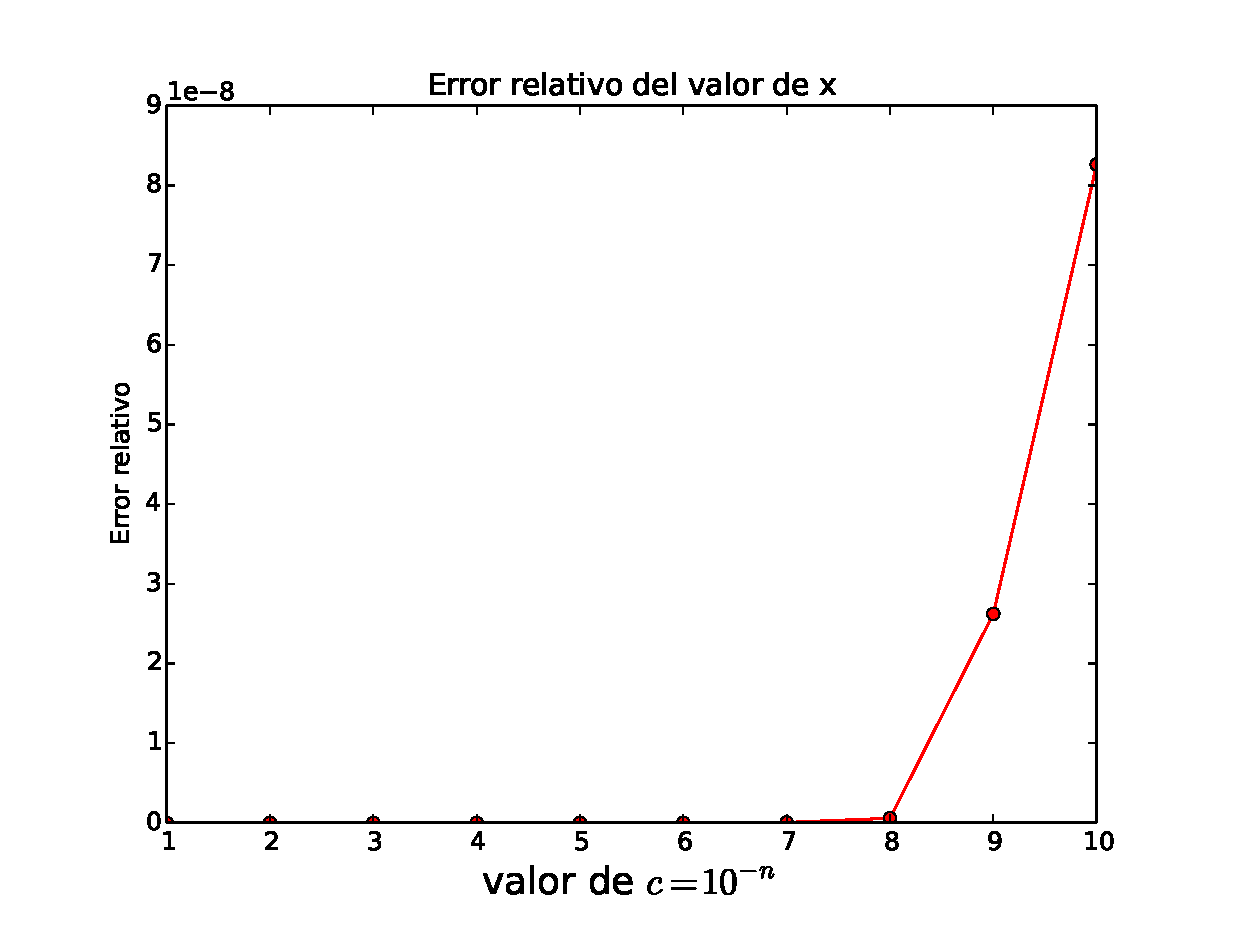
\includegraphics[scale=0.5]{Imagenes/Ejercicio_Eq_Cuadratica_01.eps}
\end{figure}
\end{frame}
\begin{frame}
\frametitle{Mejorando la gráfica}
En la gráfica anterior no es posible tener un contraste para discutir sobre el error relativo conforme el valor de $n$ aumenta, si hacemos un cambio en el eje $y$, dejándolo como un eje logarítmico con \texttt{plt.semilogy()}, tendremos:
\end{frame}
\begin{frame}
\frametitle{Mejorando la gráfica}
\begin{figure}
    \centering
    \includegraphics[scale=0.5]{Imagenes/Ejercicio_Eq_Cuadratica_02.eps}
\end{figure}
\end{frame}   
% \subsection{Ejercicio 2}
% \begin{frame}
% \frametitle{Ejercicio 2: Sumando valores}
% Del ejercicio anterior, hemos visto que la cancelación en la sustracción de los términos se presentan cuando se suma una serie con signos alternantes.
% \\
% \bigskip
% \pause
% Para una expresión veremos tres maneras distintas de hacer una suma y vamos a comparar los resultados.
% \end{frame}
% \begin{frame}
% \frametitle{Ejercicio 2: Primera suma $S^{(1)}_{N}$}
% Considera como la primera suma la expresión:
% \begin{equation}
% S^{(1)}_{N}= \sum^{2 \: N}_{n=1} (-1)^{n} \dfrac{n}{n + 1}
% \label{eq:ecuacion_02_10}
% \end{equation}
% \end{frame}
% \begin{frame}
% \frametitle{Ejercicio 2: Segunda suma $S^{(2)}_{N}$}
% Si sumamos de manera separada los valores impares y los pares de $x$, tendremos dos sumas:
% \begin{equation}
% S^{(2)}_{N}= - \sum^{N}_{n = 1} \dfrac{2 \: n-1}{2 \: n} + \sum^{N}_{n = 1} \dfrac{2 \: n}{2 \: n + 1}
% \label{eq:ecuacion_02_11}
% \end{equation}
% En esta expresión, todos los términos son positivos con sólo una sustracción al final del cálculo.
% \end{frame}
% \begin{frame}
% \frametitle{Ejercicio 2: Tercera suma $S^{(2)}_{N}$}
% Podemos eliminar la diferencia mediante una combinación entre las dos sumas anteriores, quedando de la siguiente manera
% \begin{equation}
% S^{(3)}_{N}=  \sum^{N}_{n = 1} \dfrac{1}{2 \: n \: (2 \: n + 1)}
% \label{eq:ecuacion_02_12}
% \end{equation}
% \end{frame}
% \begin{frame}
% \frametitle{Revisando las tres sumas}
% Sabemos que aunque el valor de las tres sumas $S^{(1)}_{N}$, $S^{(2)}_{N}$, $S^{(3)}_{N}$, es el mismo, el resultado númerico puede ser diferente.
% \setbeamertemplate{enumerate items}[circle]
% \begin{enumerate}[<+->]
% \item Escribe un programa que calcule $S^{(1)}_{N}$, $S^{(2)}_{N}$, $S^{(3)}_{N}$.
% \seti
% \end{enumerate}
% \end{frame}
% \begin{frame}
% \frametitle{Revisando las tres sumas}
% \setbeamercolor{item projected}{bg=blue!70!black,fg=yellow}
% \setbeamertemplate{enumerate items}[circle]
% \begin{enumerate}[<+->]
% \conti
% \item Supongamos que $S^{(3)}_{N}$ es el valor exacto de la suma. Grafica el error relativo contra el número de términos en la suma (tip: usa una escala log-log). Comienza con $N = 1$ hasta $N = 1000000$. Describe la gráfica.
% \item Identifica en tu gráfica una región en donde la tendencia es casi lineal, ¿qué representa ésta sección con respecto al error?
% \end{enumerate}
% \end{frame}
\end{document}